% ============================================================
%  Chapitre 2 — Architecture du projet
% ============================================================
\chapter{Architecture du projet}

\section{Organisation du code source}

Le projet est structuré comme un projet Maven standard avec le groupId
\code{rcr} et l'artifactId \code{projet\_RCR}.
Le code source est organisé en packages correspondant aux cinq formalismes,
plus un package \code{ui} pour l'interface graphique.

\begin{lstlisting}[style=dl, caption={Arborescence du projet Maven}]
projet_RCR/
|-- pom.xml
`-- src/main/
    |-- java/rcr/
    |   |-- Main.java                     # Entree console
    |   |-- MainApp.java                  # Entree JavaFX
    |   |-- modal/
    |   |   |-- ModalLogicMusic.java      # Kripke — musique
    |   |   `-- ModalLogicJustice.java    # Kripke — justice
    |   |-- defaut/
    |   |   |-- DefaultLogicMusic.java    # Defauts — musique
    |   |   `-- DefaultLogicJustice.java  # Defauts — justice
    |   |-- classical/
    |   |   |-- PropositionalLogicMusic.java
    |   |   |-- PropositionalLogicJustice.java
    |   |   |-- PredicateLogicMusic.java
    |   |   `-- PredicateLogicJustice.java
    |   |-- description/
    |   |   |-- DescriptionLogicMusic.java  # OWL + HermiT — musique
    |   |   `-- DescriptionLogicJustice.java
    |   |-- semantic/
    |   |   `-- SemanticNetworkExample.java
    |   `-- ui/
    |       |-- DashboardController.java
    |       |-- modal/ModalLogicController.java
    |       |-- defaut/DefaultLogicController.java
    |       |-- classical/ClassicalLogicController.java
    |       `-- description/DescriptionLogicController.java
    `-- resources/rcr/
        |-- dashboard.fxml
        `-- css/style.css
\end{lstlisting}

Chaque formalisme est développé sur une \textbf{branche Git dédiée}
(\code{logique-modale}, \code{logique-defauts}, \code{logique-classique},
\code{logique-description}), puis intégré dans la branche principale
\code{main} par un merge \emph{no fast-forward}, conformément aux
bonnes pratiques de gestion de versions.

\section{Technologies utilisées}

\begin{table}[H]
\centering
\caption{Dépendances et outils du projet}
\begin{tabularx}{\linewidth}{llX}
\toprule
\textbf{Outil / Bibliothèque} & \textbf{Version} & \textbf{Rôle} \\
\midrule
Java JDK               & 11        & Langage de programmation \\
Maven                  & 3.6+      & Gestion de projet et dépendances \\
TweetyProject          & 1.27      & Logiques modale, des défauts, classique, réseaux sémantiques \\
OWL API                & 4.5.29    & Manipulation d'ontologies OWL~2 \\
HermiT                 & 1.4.3.456 & Raisonneur OWL DL (logique de description) \\
SAT4J                  & (inclus)  & Solveur SAT pour la logique propositionnelle \\
JavaFX                 & 17.0.2    & Interface graphique \\
Git / GitHub           & ---       & Versionnement du code source \\
\bottomrule
\end{tabularx}
\end{table}

\section{Interface graphique}

L'interface graphique est réalisée en \textbf{JavaFX~17} avec une architecture
\textsc{mvc} (FXML + contrôleurs Java).
Elle adopte le thème sombre \emph{Catppuccin Mocha} et se compose d'un
\textbf{tableau de bord} (Figure~\ref{fig:dashboard}) présentant quatre cartes,
chacune ouvrant une fenêtre dédiée à un formalisme.

% --- Figure dashboard ---
\begin{figure}[H]
\centering
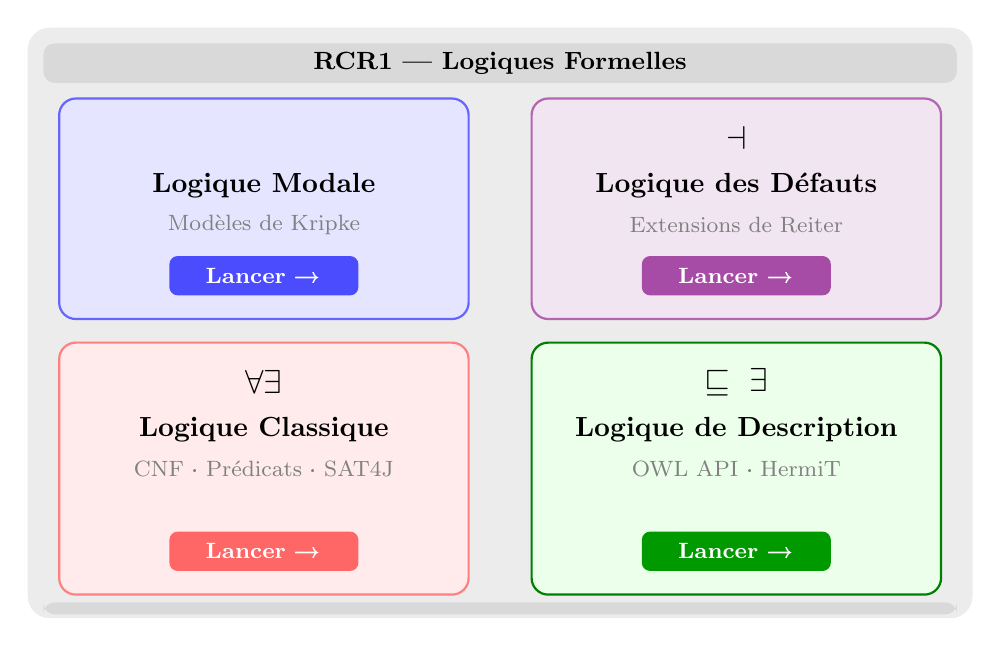
\begin{tikzpicture}[font=\small]
  % fond du dashboard
  \fill[gray!15, rounded corners=8pt] (0,0) rectangle (12,7.5);

  % header
  \fill[gray!30, rounded corners=4pt] (0.2,6.8) rectangle (11.8,7.3);
  \node at (6,7.05) {\textbf{RCR1 — Logiques Formelles}};

  % Card 1 — Modale (bleu)
  \fill[blue!10, rounded corners=6pt] (0.4,3.8) rectangle (5.6,6.6);
  \draw[blue!60, rounded corners=6pt, thick] (0.4,3.8) rectangle (5.6,6.6);
  \node[font=\large] at (3,6.1) {$\nec\;\pos$};
  \node[font=\bfseries] at (3,5.5) {Logique Modale};
  \node[align=center, font=\footnotesize, gray] at (3,5.0)
    {Modèles de Kripke};
  \fill[blue!70, rounded corners=3pt] (1.8,4.1) rectangle (4.2,4.6);
  \node[white, font=\footnotesize\bfseries] at (3,4.35) {Lancer →};

  % Card 2 — Défauts (violet)
  \fill[violet!10, rounded corners=6pt] (6.4,3.8) rectangle (11.6,6.6);
  \draw[violet!60, rounded corners=6pt, thick] (6.4,3.8) rectangle (11.6,6.6);
  \node[font=\large] at (9,6.1) {$\dashv$};
  \node[font=\bfseries] at (9,5.5) {Logique des Défauts};
  \node[align=center, font=\footnotesize, gray] at (9,5.0)
    {Extensions de Reiter};
  \fill[violet!70, rounded corners=3pt] (7.8,4.1) rectangle (10.2,4.6);
  \node[white, font=\footnotesize\bfseries] at (9,4.35) {Lancer →};

  % Card 3 — Classique (rouge)
  \fill[red!8, rounded corners=6pt] (0.4,0.3) rectangle (5.6,3.5);
  \draw[red!50, rounded corners=6pt, thick] (0.4,0.3) rectangle (5.6,3.5);
  \node[font=\large] at (3,3.0) {$\forall\exists$};
  \node[font=\bfseries] at (3,2.4) {Logique Classique};
  \node[align=center, font=\footnotesize, gray] at (3,1.9)
    {CNF · Prédicats · SAT4J};
  \fill[red!60, rounded corners=3pt] (1.8,0.6) rectangle (4.2,1.1);
  \node[white, font=\footnotesize\bfseries] at (3,0.85) {Lancer →};

  % Card 4 — Description (vert)
  \fill[green!8, rounded corners=6pt] (6.4,0.3) rectangle (11.6,3.5);
  \draw[green!50!black, rounded corners=6pt, thick] (6.4,0.3) rectangle (11.6,3.5);
  \node[font=\large] at (9,3.0) {$\sqsubseteq\;\exists$};
  \node[font=\bfseries] at (9,2.4) {Logique de Description};
  \node[align=center, font=\footnotesize, gray] at (9,1.9)
    {OWL API · HermiT};
  \fill[green!60!black, rounded corners=3pt] (7.8,0.6) rectangle (10.2,1.1);
  \node[white, font=\footnotesize\bfseries] at (9,0.85) {Lancer →};

  % footer
  \fill[gray!30, rounded corners=4pt] (0.2,0.05) rectangle (11.8,0.2);
\end{tikzpicture}
\caption{Tableau de bord JavaFX — quatre formalismes disponibles}
\label{fig:dashboard}
\end{figure}

Chaque fenêtre de formalisme propose :
\begin{itemize}
  \item Un affichage de la théorie ou de la TBox/ABox ;
  \item Un bouton de lancement du raisonneur (exécution en \emph{thread}
        d'arrière-plan pour ne pas bloquer l'interface) ;
  \item Une zone de résultats affichant la sortie du raisonneur.
\end{itemize}

\section{Lancement du projet}

\begin{lstlisting}[style=dl, caption={Commandes de lancement}]
# Aller dans le repertoire du projet
cd projet_RCR

# Interface graphique JavaFX
mvn javafx:run

# Mode console (tous les formalismes)
mvn exec:java

# Formalisme specifique
mvn exec:java -Dexec.mainClass="rcr.description.DescriptionLogicMusic"
\end{lstlisting}
